% Minimal sentence-level revisions: C-61 to C-97 and the specified global edits.
\section{\src{Random forest}}\label{sec:forest}
\subsection{\src{Method, tuning and test predictions}}\label{sec:forest-method}

\src{\textbf{Method.} The first model is a random forest. Because our study is a classification problem, a random forest appeared a promising starting point (Batsuuri et al., 2024, p. 3). This model combines many classification trees, each splitting the data through a series of simple yes/no questions.}

\src{A single tree captures non-linear patterns and interactions, but it is unstable: small changes in the data can produce a very different tree. For this reason, we use bagging (bootstrap aggregation). The idea is to grow many trees, each on a bootstrap sample (programmes drawn with replacement), and average their votes. Averaging helps to cancel out noisy predictions. However, bagging alone has a weakness. If one input is very strong, almost every tree will split on it first, making the trees similar, which limits the gain from averaging (James et al., 2013, p. 320). Indeed, Hastie et al. (2009, p. 588) formalised it with the variance of an average of B trees, each with variance σ² and pairwise correlation ρ:}

\begin{equation}
\label{eq:forest-variance}
\operatorname{Var}=\rho\sigma^2+\frac{(1-\rho)\sigma^2}{B}
\end{equation}

\src{More trees (B) shrink the second term, but the first term only shrinks with less correlated trees. We use Breiman’s (2001a, p. 6) solution of limiting each split to a random subset of \emph{mtry} inputs. Each tree then votes: the share of trees voting “interrupted” gives the predicted probability, and a threshold assigns the class. The programmes left out of each bootstrap sample (out-of-bag, OOB) provide a built-in error estimate.}

\src{\textbf{Default forest.} The default forest was trained with the default hyperparameters of the \emph{randomForest} R package (Liaw \& Wiener, 2002): 500 trees, \emph{mtry} 3. Its OOB balanced accuracy is 0.609.}

\src{\textbf{Hyperparameter tuning.} To tune our hyperparameters (number of trees and \emph{mtry}), we scored 24 different pairs on balanced accuracy (Section~\ref{sec:prediction-task}), ranging from 100 to 1000 trees and \emph{mtry} from 2 to 12, with the \emph{caret} package (Kuhn, 2008).}

\src{We used three different cross-validation schemes: 10-fold CV, LOOCV and country-grouped 10-fold CV (country CV, Section~\ref{sec:data-sources}). The last is our main measurement, as it keeps all programmes of a country in the same fold, so the forest is never scored on a country it was trained on.}

\src{For 10-fold CV and country CV, we compute balanced accuracy within each fold and average over the ten folds; for LOOCV, where each fold holds a single programme, we compute it once over all out-of-fold predictions. Table~\ref{tab:rf-tuning} compares the default forest with the best pair under each scheme.}

\begin{wordtable}
\begin{tabularx}{\linewidth}{@{}>{\raggedright\arraybackslash}XL{0.22\linewidth}>{\raggedright\arraybackslash}XL{0.22\linewidth}@{}}
\toprule
\textbf{\src{Validation scheme}} & \textbf{\src{Default forest (500 trees, \emph{mtry} 3)}} & \textbf{\src{Best pair under this scheme}} & \textbf{\src{Balanced accuracy of best pair}}\\
\midrule
\src{Out-of-bag (default forest only)} & \src{0.609} & \src{n/a} & \src{n/a}\\
\src{10-fold CV} & \src{0.623} & \src{250 trees, \emph{mtry} 2} & \src{0.657}\\
\src{Country-grouped 10-fold CV} & \src{0.597} & \src{250 trees, \emph{mtry} 3} & \src{0.620}\\
\src{LOOCV} & \src{0.606} & \src{100 trees, \emph{mtry} 8} & \src{0.635}\\
\bottomrule
\end{tabularx}
\wordtablecaption{tab:rf-tuning}{\src{Table \thetable. Default against tuned forest on the training set (balanced accuracy; best of 24 pairs per scheme)}}
\end{wordtable}

\src{The default pair (500, 3) is part of the tuning grid, so its CV scores come from the same runs. OOB accuracy of the default forest is 0.628.}

\src{Country CV gives the lowest best score (0.620, against 0.657 for 10-fold CV and 0.635 for LOOCV), as expected, since the forest is never tested on a country it has seen. We still select it because it guards against within-country dependence (Section~\ref{sec:data-sources}), although 26 of the 28 test programmes come from countries seen in training, so it does not imitate the later-period test.}

\src{\textbf{Final model.} We keep the pair chosen under country CV (250 trees, \emph{mtry} 3), refit it on all 145 training programmes with the threshold that maximises out-of-fold balanced accuracy (0.51), and predict the 28 test programmes once (Table~\ref{tab:rf-results}). The selected pair keeps the default \emph{mtry} and only lowers the number of trees from 500 to 250, which cannot be expected to improve accuracy, so its gain over the default under country CV (0.620 against 0.597) most likely reflects noise in a search over 24 pairs. Only the test-set rows of Table~\ref{tab:rf-results} measure out-of-sample performance; the other figures in Tables~\ref{tab:rf-tuning} and~\ref{tab:rf-results} are training-set estimates used to choose settings.}

\begin{wordtable}
\begin{tabularx}{\linewidth}{@{}>{\raggedright\arraybackslash}XL{0.115\linewidth}L{0.12\linewidth}L{0.12\linewidth}L{0.13\linewidth}r@{}}
\toprule
\textbf{\src{Model}} & \textbf{\src{Accuracy}} & \textbf{\src{Sensitivity}} & \textbf{\src{Specificity}} & \textbf{\src{Balanced accuracy}} & \textbf{\src{AUC}}\\
\midrule
\src{Baseline (always interrupted)} & \src{0.607} & \src{1.000} & \src{0.000} & \src{0.500} & \src{0.500}\\
\addlinespace
\src{Default forest (threshold 0.50)} & \src{0.571} & \src{0.588} & \src{0.545} & \src{0.567} & \src{0.620}\\
\addlinespace
\src{Final forest (threshold 0.51)} & \src{0.500} & \src{0.471} & \src{0.545} & \src{0.508} & \src{0.586}\\
\addlinespace
\src{Final forest (threshold 0.50)}\footnotemark[1] & \src{0.571} & \src{0.588} & \src{0.545} & \src{0.567} & \src{0.586}\\
\midrule
\src{Final forest, training out-of-fold (\emph{n} = 145, threshold 0.51)} & \src{0.641} & \src{0.523} & \src{0.738} & \src{0.630} & \src{0.631}\\
\bottomrule
\end{tabularx}
\wordtablecaption{tab:rf-results}{\src{Table \thetable. Random forest on the test set (28 programmes, 2014–2016), with the final forest’s training out-of-fold scores for reference}}
\end{wordtable}
\footnotetext[1]{\srcnote{Note. Final forest: 250 trees, \emph{mtry} 3. The 0.50 row uses the same threshold as the logistic regression, for a like-for-like comparison; it differs from 0.51 only because two interrupted programmes sit at a vote share of 0.504. The last row is computed on the 145 training programmes, not on the test set.}}

\src{\textbf{Out-of-sample predictions.} On the 28 test programmes, the final forest reaches a balanced accuracy of 0.508, barely above the 0.500 of always predicting “interrupted”, and its accuracy (0.500) is even below that rule’s (0.607); the rule’s high accuracy despite zero skill shows why plain accuracy misleads when classes are unequal. Out of fold on the training set, it reaches 0.630; this is more precise than the test score but slightly optimistic, since both the pair and the threshold were chosen on these predictions. It differs from the 0.620 in Table~\ref{tab:rf-tuning} because that figure averages balanced accuracy over ten folds at threshold 0.50, whereas 0.630 pools all out-of-fold predictions at threshold 0.51. The default forest’s higher test balanced accuracy (0.567 against 0.508) comes entirely from two interrupted programmes with a vote share of 0.504: they are classed as interrupted at threshold 0.50 but as completed at 0.51, and at 0.50 the final forest also scores 0.567. The default forest also ranks programmes better (AUC 0.620 against 0.586), so tuning did not improve the test results on either measure. On the test set, one extra correct prediction moves balanced accuracy by about 0.03 to 0.05. The forest thus finds a modest signal in the training set, but no reliable advantage over chance on later programmes.}

\src{Random forests are considered black-box models because hundreds of trees cannot be read directly. However, the contribution of each input can still be measured, as explained in Section~\ref{sec:importance}.}

\subsection{\src{Variable importance}}\label{sec:importance}

\src{Permutation importance shuffles the values of each input among the out-of-bag samples, breaking its link with the target, and measures the resulting drop in accuracy, averaged over all trees. Higher values mean higher predictive power, while small or negative values signal no contribution. The mean decrease in accuracy (MDA) is one of the two importance measures in \emph{randomForest}, the other being the mean decrease in Gini impurity (Abedin et al., 2021, p. 23). Importance indicates neither direction nor causality, and correlated inputs (the extended and concessional indicators) share credit.}

\begin{wordtable}
\centering
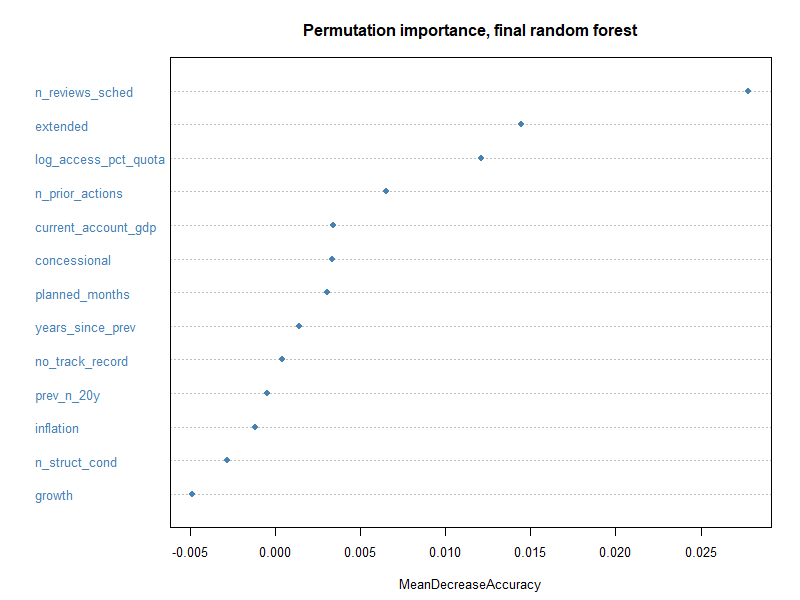
\includegraphics[width=0.82\linewidth]{../Presentation/figures/rf_importance.png}
\refstepcounter{figure}\label{fig:rf-importance}
\wordcaption{\src{Figure \thefigure. Permutation importance of the final forest: mean decrease in out-of-bag accuracy when one input is shuffled (higher values mean more important; values near or below zero mean no contribution)}}
\end{wordtable}

\src{The number of scheduled reviews is the strongest input (Figure~\ref{fig:rf-importance}): 85\% of training programmes with eight or more reviews were interrupted, against 36\% of the others. Part of this is mechanical, as each extra review is one more chance to miss one (Section~\ref{sec:variables}). Because this link is partly built into the outcome, the forest’s training-set signal should be read as an upper bound on what approval-day information reveals about implementation. Programme length receives little importance on its own because it overlaps with the extended indicator (\emph{r} = 0.77); within each facility type, longer training programmes were interrupted more often (all 10 non-extended programmes planned for more than 30 months, against 49\% of those planned for 30 months or less), in line with Reinsberg et al. (2022, p. 1028), who find that longer agreements fail more often. Extended facilities (EFF or ECF) come second, with 38\% of extended training programmes interrupted against 60\% of the others, in line with the IMF’s review: “EFF and EFF-ECF arrangements, generally longer in duration than SBAs, had higher completion rates” (IMF, 2019, p. 45). In our sample the gap mainly reflects ECFs (36\% of training ECFs interrupted), which are also concessional; EFFs alone (57\%) differ little from SBAs (60\%). Section~\ref{sec:policy} discusses whether higher completion in extended programmes reflects better implementation. Access relative to quota ranks third and prior actions fourth (48\% interrupted with at least one prior action, against 37\% without), in line with the IMF’s finding of “a negative association between PAs [prior actions] at arrangement approval and completion rates” (IMF, 2019, p. 45).}

\src{Growth and inflation add no predictive value. Several regression studies find initial economic conditions largely insignificant (Ivanova et al., 2003, p. 1; Reinsberg et al., 2022, p. 1028), although Dreher (2003) reports associations with initial economic vulnerability, and our macro inputs are staff projections, which may be optimistic (Section~\ref{sec:variables}). The literature disagrees on conditionality: Reinsberg et al. (2022, p. 1028) find that structural conditions are associated with interruption, while Ivanova et al. (2003, p. 1) find no material effect. A simple count of structural conditions adds no predictive value in our forest, which therefore cannot test Reinsberg et al.’s finding on specific condition types. These importances describe patterns in the training sample that did not carry over clearly to the test period, and most values outside the top three are close to zero. Section~\ref{sec:alternatives} asks whether a simpler or a more flexible model does better.}
